\documentclass[aspectratio=169,11pt]{beamer}
\usetheme{default}
\usecolortheme{default}
\setbeamertemplate{navigation symbols}{}
\setbeamertemplate{footline}[frame number]
\usepackage{graphicx}
\usepackage{booktabs}
\definecolor{cont}{HTML}{2A78B5}
\definecolor{vm}{HTML}{D9822B}
\setbeamercolor{frametitle}{fg=cont}
\setbeamercolor{title}{fg=cont}
\newcommand{\C}[1]{\textcolor{cont}{\textbf{#1}}}
\newcommand{\V}[1]{\textcolor{vm}{\textbf{#1}}}

\title{Virtual Machines vs.\ Containers}
\subtitle{Same Web API, Same Host, Same Limits --- What Really Differs?}
\author{Soner Yan\i k \quad B2305.010151}
\institute{SEN421 Cloud Architecture and Services --- Topic 2, Part A\\Istanbul Ayd\i n University}
\date{Fall 2026}

\begin{document}

\begin{frame}
	\titlepage
\end{frame}

\begin{frame}{The question}
	\begin{itemize}
		\item Every cloud workload needs isolation: \V{VM} (own kernel, hypervisor) or \C{container} (shared kernel).
		\item The choice decides how fast we scale, how densely we pack servers and what we pay.
	\end{itemize}
	\vspace{0.4cm}
	\begin{block}{Research question}
		For the same small web API with 2 vCPU and 2 GB, how do a container and a VM differ in
		\textbf{image size, startup time, memory} and \textbf{requests per second} --- and why?
	\end{block}
	\vspace{0.3cm}
	My guess before measuring: container \textbf{$\sim$10$\times$ faster}, \textbf{$\sim$2$\times$ less memory}.
\end{frame}

\begin{frame}{Design}
	\begin{columns}[c]
		\column{0.62\textwidth}
		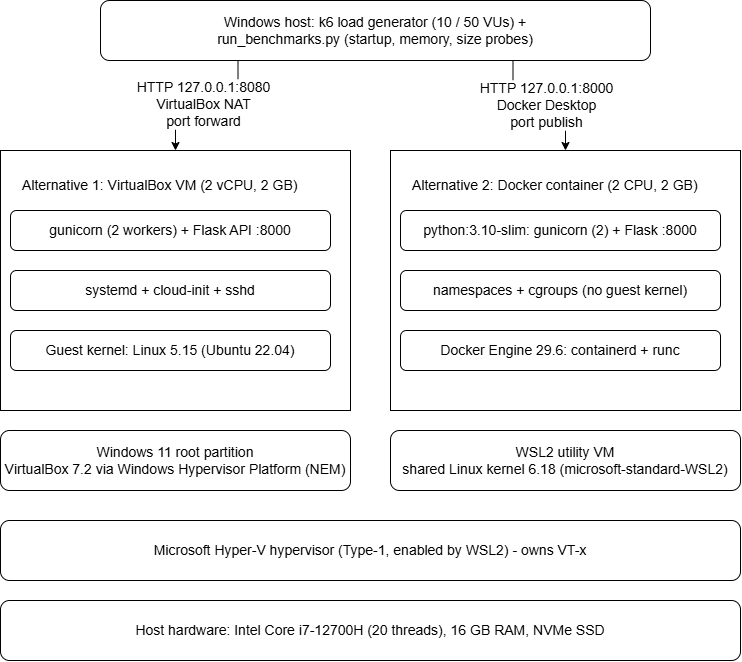
\includegraphics[width=\linewidth]{figures/fig_architecture_drawn.png}
		\column{0.38\textwidth}
		\small
		\begin{itemize}
			\item Flask API + gunicorn (2 workers): \texttt{/hello}, \texttt{/compute}, \texttt{/health}
			\item \V{VM}: VirtualBox 7.2, Ubuntu 22.04, kernel 5.15
			\item \C{Container}: Docker 29.6, WSL2 kernel 6.18
			\item \textbf{Control}: container with the VM's exact Ubuntu, Python and OpenSSL
			\item Hyper-V sits under \emph{both}
		\end{itemize}
	\end{columns}
\end{frame}

\begin{frame}{Method}
	\begin{itemize}
		\item One script runs every measurement --- only one alternative running at a time
		\item \textbf{Startup}: start command $\rightarrow$ first HTTP 200 on \texttt{/health}, 5 successful cold starts
		\item \textbf{Memory}: \texttt{docker stats} vs.\ guest \texttt{free} + VirtualBox process on Windows
		\item \textbf{Load}: k6, 10 and 50 virtual users, 30 s, 3 runs per configuration
		\item \textbf{Pure CPU}: 200k SHA-256 rounds without HTTP
		\item Laptop: i7-12700H, 16 GB, Windows 11 --- cost: \textbf{0 USD}, all local
	\end{itemize}
\end{frame}

\begin{frame}{Results: startup and memory}
	\begin{columns}[t]
		\column{0.5\textwidth}
		\centering
		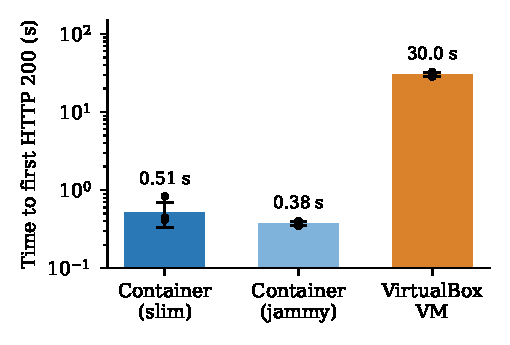
\includegraphics[width=\linewidth]{figures/fig_startup.pdf}\\
		\small \C{0.4--0.5 s} vs.\ \V{30 s} $\Rightarrow$ $\sim$60$\times$\\
		\textbf{8 of 13 VM boots hung}
		\column{0.5\textwidth}
		\centering
		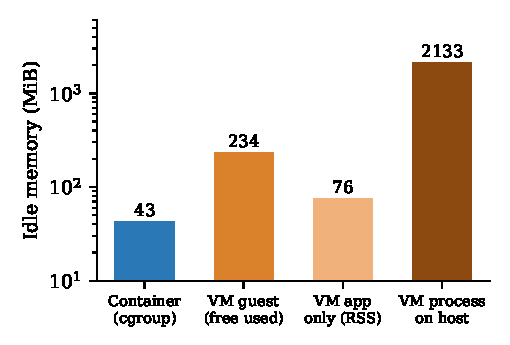
\includegraphics[width=\linewidth]{figures/fig_memory.pdf}\\
		\small \C{43 MiB} vs.\ \V{234 MiB} in guest, \V{2.1 GiB} reserved\\
		Image: \C{202 MB} vs.\ \V{2.7 GB} ($\sim$13$\times$)
	\end{columns}
\end{frame}

\begin{frame}{Results: throughput --- and a hypothesis that failed}
	\begin{columns}[c]
		\column{0.5\textwidth}
		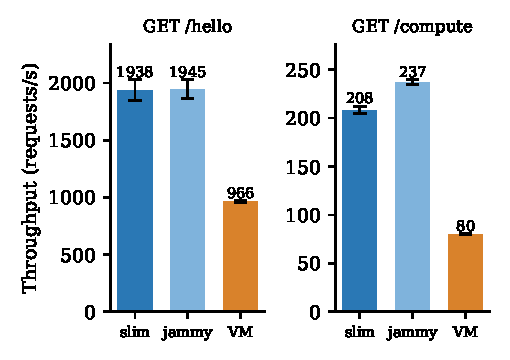
\includegraphics[width=\linewidth]{figures/fig_throughput.pdf}
		\column{0.5\textwidth}
		\small
		\begin{itemize}
			\item 10 VUs: VM gives \V{50\%} of container on \texttt{/hello}, \V{34--38\%} on \texttt{/compute}
			\item 50 VUs: \V{48\% errors} on VM \texttt{/hello} $\rightarrow$ VirtualBox NAT, not the app
			\item Hypothesis: older OpenSSL in VM causes CPU gap
			\item Control container with \emph{same} OpenSSL: still fast (237 req/s)
			\item $\Rightarrow$ gap comes from the \textbf{virtualization layer}
		\end{itemize}
	\end{columns}
\end{frame}

\begin{frame}{Cost and security}
	\begin{columns}[t]
		\column{0.5\textwidth}
		\textbf{Cost} (Azure list prices, 22 Nov 2026)\\[0.2cm]
		\small 8 isolated services, per month:\\[0.1cm]
		\begin{tabular}{lr}
			\toprule
			8 $\times$ B2s VM & \V{\$280} \\
			1 $\times$ D4s\_v5 + 8 containers & \C{\$168} \\
			\bottomrule
		\end{tabular}\\[0.2cm]
		$\Rightarrow$ $\sim$\textbf{40\% cheaper}\\
		Experiments: \textbf{0 USD}
		\column{0.5\textwidth}
		\textbf{Security / responsibility}\\[0.2cm]
		\small
		\begin{itemize}
			\item \V{VM}: separate kernel = stronger boundary
			\item \C{Container}: one shared kernel for all tenants
			\item Cloud: provider $\rightarrow$ hardware, hypervisor (+ host kernel if managed); me $\rightarrow$ image, patches, secrets, ports
			\item To fix before production: run container as non-root, publish port on 127.0.0.1 only
		\end{itemize}
	\end{columns}
\end{frame}

\begin{frame}{Lessons and recommendation}
	\begin{itemize}
		\item Guess vs.\ reality: startup \textbf{60$\times$} (not 10), memory \textbf{5--50$\times$} (not 2), throughput \textbf{2--3$\times$} (not 10)
		\item \C{Containers} for many small, stateless services that must scale fast
		\item \V{VMs} when strong kernel isolation or another OS is needed
		\item Biggest surprise: the \textbf{nested Hyper-V + VirtualBox} setup, not virtualization itself, caused the worst penalties
		\item Always test a hypothesis with a control experiment
		\item Next: repeat on Linux/KVM and in a cloud autoscaling group
	\end{itemize}
	\vfill
	\centering\small Code and data: github.com/soneryanik/cloud-vm-container-test
\end{frame}

\end{document}
